\section{Problem Formulation}\label{sec:problem-formulation}

We focus on the robotic grasping of visually-perceived objects within the reachable workspace. It is assumed that any previous or subsequent motion of the rover and its arm is performed by traditional methods or other policies that are part of a larger hierarchy. We do not distinguish between isolated objects and those in cluttered scenes because rovers in extraterrestrial conditions would encounter both cases. We consider the task to be episodic, where each episode is successful once an object is grasped and lifted above a required threshold. Due to uneven terrain, this requirement is specified to be~25~cm above the base footprint of the robot. Each episode is further limited to~40~s, meaning that termination with failure occurs after a corresponding number of steps without success.

The task of robotic grasping can be formulated as a Markov decision process, where the behavior of an agent is defined by a policy~\mbox{\(\pi:\mathcal{S}\rightarrow\mathcal{A}\)} that provides a mapping from states to actions. At each discrete time step~\(t\), the environment utilizes a reward function~\mbox{\(r(s_{t},a_{t})\!\in\!\mathbb{R}\)} to emit an immediate reward for executing an action~\(a_{t}\) in a state~\(s_{t}\), which brings the agent to the next state~\(s_{t+1}\). The primary objective of the agent is to find the optimal policy~\(\pi^{*}\) that maximizes the expected sum of all future rewards~\mbox{\(\sum_{i=t}^T \gamma^{i-t}r(s_{i},a_{i})\)}, which are discounted by~\mbox{\(\gamma\!\in\![0, 1]\)} over a time horizon. Due to our focus on episodic grasping,~\(T\) indicates the terminal state of an episode.

\begin{figure*}[thpb]
	\vspace{1.379mm}
	\centering
	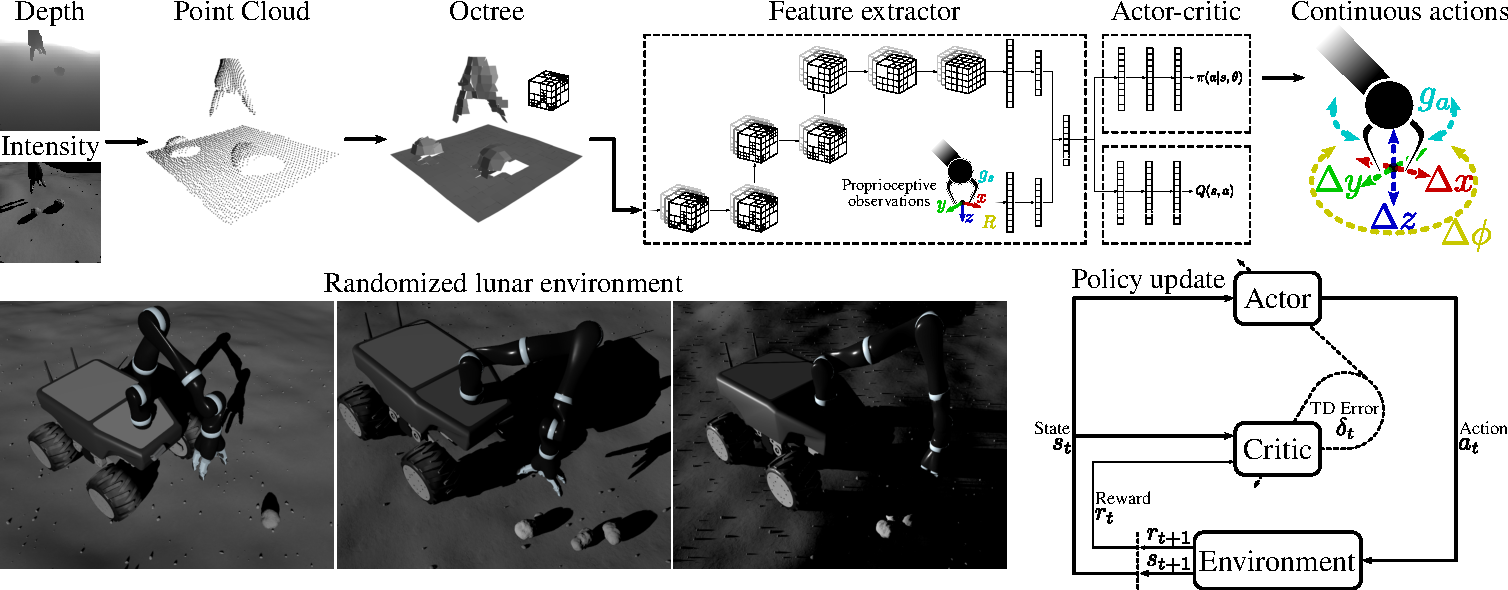
\includegraphics[width=1.0\textwidth]{system_overview.pdf}
	\caption{Overview of our approach for training reinforcement learning agents using a model-free actor-critic algorithm in lunar environments. For visual observations, we employ octrees that are constructed from depth maps and monochromatic images via an intermediate representation in the form of point clouds. Together with proprioceptive observations, a shared feature extractor is utilized to provide abstract features that are used as input for both actor and critic networks. The actor network optimizes a stochastic policy that provides continuous actions in Cartesian space in the form of gripper displacement and action. All of these networks are optimized simultaneously via end-to-end learning while an agent is trained inside a randomized simulation environment.}
	\label{fig:system-overview}
\end{figure*}

\section{Learning to Grasp from Octree Observations}\label{sec:learning-to-grasp-from-octree-observations}

Our approach incorporates visual octree observations with end-to-end learning of robotic grasping in a procedurally-generated simulation environment. An overview of the approach is presented in Fig.~\ref{fig:system-overview}.

\subsection{Truncated Quantile Critics}\label{ssec:truncated-quantile-critics}

We use Truncated Quantile Critics (TQC)~\cite{kuznetsov_controlling_2020} in this work to learn a policy for robotic grasping. It is a model-free off-policy actor-critic algorithm that incorporates both an actor for optimizing a stochastic policy~\mbox{\(\pi(a \vert s, \theta)\)} parameterized by \(\theta\), and one or more critics to estimate the action-value function~\mbox{\(Q(s, a)\)} by iteratively minimizing the temporal difference error \(\delta_{t}\) for a set of all available continuous actions that the agent is allowed to take. Critics evaluate the actor based on how rewarding the selected actions are. TQC is an extension of Soft Actor-Critic (SAC)~\cite{haarnoja_soft_2018} and therefore employs entropy regularization to optimize a trade-off between expected return and entropy, which represents the randomness of the policy. Unlike SAC, TQC utilizes a distributional representation for the action-value function~\mbox{\(Q(s, a)\)} of critics and truncates a number of topmost atoms from such distributions to address the problems with overestimation. We employ the specific implementation of TQC from Stable Baselines3~\cite{raffin_stable-baselines3_2021}.

\subsection{Observation Space}\label{ssec:observation-space}

The observation space of the agent consists primarily of visual observations that are represented as 3D octrees. Visual data originates from a stereo camera that is considered to be a space-suitable sensor as it is already used onboard current rovers~\cite{grotzinger_mars_2012}. In addition to depth maps produced by the camera, we also use monochromatic images captured by one of the imaging sensors to provide agents with supplementary information about the scene, e.g. the notion of shadows, as visualized in Fig.~\ref{fig:system-overview}. No meaningful information would be gained from multi-channel color images because lunar environments are generally homogeneously colored. Proprioceptive observations are also included to provide information about the state of the gripper in the case it is occluded or outside of the camera view. Only the gripper pose~\mbox{\((x,y,z,R_{1},R_{2},R_{3},R_{4},R_{5},R_{6})\)} and its state~\mbox{\(g_{s}\!\in\!\{closed\!:-1,open\!:1\}\)} are used in order to keep the observation space invariant to the utilized robot. Gripper pose is represented with respect to the robot base, and its orientation \(R\) is expressed as a continuous 6D rotation representation from~\cite{zhou_continuity_2019} due to its suitability for deep learning. Furthermore, the last two observations are stacked together at each time step, similar to the image stacking method presented in~\cite{mnih_human-level_2015}. This promotes the Markov property of the decision process formulation by providing the agent with temporal information about environment states and dynamics, such as the notion of motion.

Conversion of visual observations to octrees begins with the aforementioned depth map and monochromatic image, which are used to create a point cloud of the scene in the form of an unstructured list of~\mbox{\((x,y,z,i)\)} tuples. This intermediate representation is then transformed into the coordinate frame of the robot base. Such transformation between the camera and robot is assumed to be known or estimated via a hand-eye calibration procedure. Once transformed, the point cloud is cropped to occupy a fixed volume in space with a uniform aspect ratio. All remaining points are then used to construct an octree by performing a recursive subdivision of the occupied 3D volume until a certain depth~\(d_{max}\) is reached. Contrary to the inefficiency of voxel grids, octrees create hierarchical tree-like data structures where only occupied cells are recursively decomposed into eight child octants. Observable features can then be stored as channels at the finest leaf octants of the new octree, i.e.~the smallest possible octants at depth~\(d_{max}\). For each of these octants, all points from the point cloud that occupy the same volume in space are used to extract the relevant features. We store three distinct attributes at each finest leaf octant, i.e.~the average unit normal vector~\mbox{\((\overline{n}_{x},\overline{n}_{y},\overline{n}_{z})\)} estimated from the points, the average distance~\(\overline{d}\) from the center of an octant cell to all points used during its formation, and the average intensity~\(\overline{i}\). Both~\(\overline{d}\) and~\(\overline{i}\) are normalized to be in the range~\([0,1]\).

\subsection{Action Space}\label{ssec:action-space}

The agent is allowed to control the motion of the robotic arm at each time step through continuous actions in Cartesian space. These were selected in favor of joint commands due to their invariance to the specific kinematic configuration of the utilized robot. As illustrated in Fig.~\ref{fig:system-overview}, the action space for control of the gripper pose incorporates the relative translation~\mbox{\((\Delta{x},\Delta{y},\Delta{z})\!\in\![-1,1]\)} and yaw rotation~\mbox{\(\Delta{\phi}\!\in\![-1,1]\)}, which are expressed with respect to the robot base frame. Prior to executing these actions, they are mapped to their respective metric and angular ranges of \(\pm\)10~cm and \(\pm\)45\textdegree. Traditional collision-free motion planning and execution are accomplished by MoveIt~2~\cite{moveit2} while utilizing \mbox{TRAC-IK}~\cite{beeson_trac-ik_2015} kinematics solver and \mbox{RRTConnect}~\cite{kuffner_rrt-connect_2000} for path planning. Control of the gripper is similarly accomplished via a continuous action~\mbox{\(g_{a}\!\in\![-1,1]\)}, where positive values open and negative values close the gripper. The control frequency of the agent is set to 2.5~Hz because it is designed to provide high-level decision-making commands, while the lower-level controllers running at 200~Hz in simulation and 500~Hz on the real robot are responsible for real-time execution. With the aforementioned limitation of~40~s, this results in a maximum of~100 discrete time steps per episode during which the agent can select its actions.

\begin{figure*}[thpb]
	\vspace{1.379mm}
	\centering
	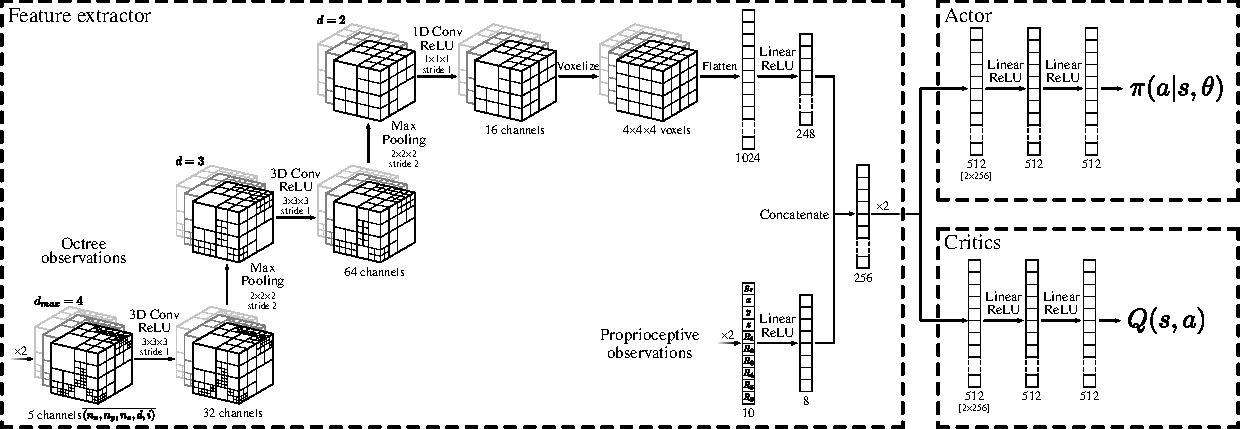
\includegraphics[width=1.0\textwidth]{actor_critic_network_full.pdf}
	\caption{The full network architecture with a shared octree-based feature extractor and separate actor-critic networks.}
	\label{fig:actor-critic-network}
\end{figure*}

\subsection{Composite Reward Function}\label{ssec:composite-reward-function}

To accelerate training, we use a composite reward function that combines sparse rewards from four distinct stages of the entire grasping task, i.e.~reaching, touching, grasping and lifting. These follow a hierarchical flow, where each stage can give a reward upon its completion only once per episode. Their corresponding reward is set to increase exponentially as~\mbox{\(r_{b}^{r_{i}-1}\)} based on their order~\mbox{\(r_{i}\!\in\![1,4]\)} in the hierarchy. The base of the exponential function can be tuned, where~\mbox{\(r_{b}\!=\!8\)} was selected for TQC through empirical evaluation. This results in a theoretical maximum reward of~585 for each successful episode. In addition to the composite reward, a small reward of~\(-0.1\) is subtracted at each time step until the termination in order to encourage the agent to accomplish the task as fast as possible.

\subsection{End-to-End Learning from Octrees}\label{ssec:end-to-end-learning-from-octrees}

We employ a novel end-to-end approach for learning a policy that maps 3D octree observations directly into continuous actions via function approximation in the form of neural networks that are visualized in Fig.~\ref{fig:actor-critic-network}. Even though TQC requires separate networks for the actor and critics, it is beneficial to share a portion of their networks to reduce the total number of learnable parameters when dealing with high-dimensional visual observations such as octrees. Therefore, we adapt the octree-based convolutional neural network architecture from~\cite{wang_o-cnn_2017} into a feature extracting module that is optimized simultaneously with the actor and critic networks during the training. We utilize octrees with a maximum depth of~\mbox{\(d_{max}=4\)} as the input, which are processed through a series of 3D convolutional and pooling layers that progressively increase the number of channels while reducing the depth of the octree. In order to enable the use of standard network layers that operate on data structures with a fixed size, each octree is voxelized after reaching the depth~\mbox{\(d=2\)} by assigning zeros to all channels of every empty cell. Visual and proprioceptive features are then concatenated together into a feature vector. The feature extractor is applied in parallel to the entire temporally-stacked observation as a part of the same mini-batch. The output of this operation is then concatenated into a single feature vector that is used as input for the separate actor-critic networks that comprise of fully-connected layers.

\subsection{Training Environment}\label{ssec:training-environment}

We create a new simulation environment for the training of agents under lunar conditions. Our environment provides a standardized OpenAI Gym~\cite{brockman_openai_2016} interface while utilizing Gazebo~\cite{gazebo} robotics simulator (formerly known as Ignition). Gazebo was selected due to its open-source nature that encourages reproducibility and plugin-based architecture that makes it easily extensible. We employ DART physics engine with a step size of 5~ms to simulate rigid-body dynamics. Furthermore, physically-based rendering (PBR) capabilities are facilitated by using OGRE~2. Gym-Ignition~\cite{ferigo_gym-ignition_2020} is utilized for interfacing Gazebo due to its focus on reinforcement learning research. Lastly, ROS~2~\cite{ros2} is used as the middleware to facilitate communication among the primary nodes while simplifying the sim-to-real transfer by providing an identical interface for both simulated and real robots.

Datasets of models for terrain and objects are necessary to simulate a realistic-looking lunar environment that encapsulates its variety. However, there is a lack of available datasets from this domain that would provide the required level of detail at the scale of the robot workspace. For this reason, we create our datasets for both lunar surfaces and rocks through procedural generation. Our synthetic mesh generation pipelines are based on the Geometry Nodes feature of Blender~\cite{blender}. For each model, we apply displacement to individual vertices by a randomized 3D pattern that is formed as a combination of multiple random procedural textures at different scales. For lunar terrain, a subdivided 2D plane is used as the original geometry while imitating uneven terrain with impact craters. Lunar rocks are initialized from subdivided convex polyhedrons that are displaced to represent rocks of different sizes and shapes, including non-convex geometry. To improve training times, each model is generated at two different levels of detail, where a simpler one is used for its collision geometry. Furthermore, each model is assigned a random set of PBR material textures during its insertion into the environment. Using this simple technique, we can synthesize unique environments with nearly an unlimited number of permutations. During our experiments, we utilize a dataset with 250~surfaces, 250~rocks and 35~PBR texture sets.

Domain randomization is employed in order to increase the variety of the environment even further, which is illustrated by the initial states of three example episodes in Fig.~\ref{fig:system-overview}. The following attributes are randomized from uniform distribution during environment resets:~the pose of the rover within the environment and the initial joint configuration of its arm above the workspace; terrain model, its surface friction and material; object count~(1~--~4), their models, densities, surface frictions, materials and poses relative to the rover; as well as direction and elevation of the simulated Sun. The pose of the virtual camera is also randomized relative to its mounting surface on the rover~(\(\pm\)5 cm). Furthermore, Gaussian noise~\mbox{\(\mathcal{N}(0, 0.001)\)} is added to the captured depth maps and monochromatic images in order to increase the realism of observations.

\subsection{Curriculum}\label{ssec:curriculum}

In order to accelerate the training in the early stages, a curriculum is applied to the height requirement for the successful lifting of objects. This requirement is set to be proportional to the current success rate smoothed by a rolling average over the last~100 episodes. The requirement is initialized at 7.5~cm and increased linearly to 25~cm until a success rate of 33\% is reached. With this addition, successful grasps become more common during the early stages of training while the actions of agents are nearly random.
